\documentclass[12pt,compress,aspectratio=169]{beamer}
\usetheme{metropolis}
\setbeamersize{text margin left=.5cm,text margin right=.5cm}
\usepackage[lf]{carlito}
\usepackage{siunitx}
\usepackage{tikz}
\usepackage{mathpazo}
\usepackage{bm}
\usepackage{mathtools}
\usepackage[ISO]{diffcoeff}
\diffdef{}{ op-symbol=\mathsf{d} }
\usepackage{xcolor,colortbl}

\setmonofont{Ubuntu Mono}
\setlength{\parskip}{0pt}
\renewcommand{\baselinestretch}{1}

\sisetup{
  inter-unit-product=\cdot,
  per-mode=symbol
}

\tikzset{
  >=latex
}

%\newcommand{\iii}{\hat{\bm\imath}}
%\newcommand{\jjj}{\hat{\bm\jmath}}
%\newcommand{\kkk}{\hat{\bm k}}


\usetikzlibrary{patterns}

\title{Class 7: Rotational Motion of a Rigid Body}
\subtitle{Advanced Placement Physics C}
\author[TML]{Dr.\ Timothy Leung}
\institute{Olympiads School}
\date{Updated: Summer 2022}

\newcommand{\pic}[2]{
  \includegraphics[width=#1\textwidth]{#2}
}
\newcommand{\eq}[2]{
  \vspace{#1}{\Large
    \begin{displaymath}
      #2
    \end{displaymath}
  }
}
%\newcommand{\iii}{\ensuremath\hat{\bm{\imath}}}
%\newcommand{\jjj}{\ensuremath\hat{\bm{\jmath}}}
%\newcommand{\kkk}{\ensuremath\hat{\bm{k}}}
\newcommand{\iii}{\ensuremath\hat\imath}
\newcommand{\jjj}{\ensuremath\hat\jmath}
\newcommand{\kkk}{\ensuremath\hat k}


\begin{document}

\begin{frame}
  \maketitle
\end{frame}


\section{Introduction}

\begin{frame}{Uniform Circular Motion}
  Consider the uniform circular motion of an object with (constant) angular
  velocity $\vec\omega$. If the rotation is counterclockwise, the direction of
  $\vec\omega$ is \emph{out of the page}; if rotation is clockwise,
  $\vec\omega$ is \emph{into the page}.
  \begin{columns}
    \column{.3\textwidth}
    \centering
    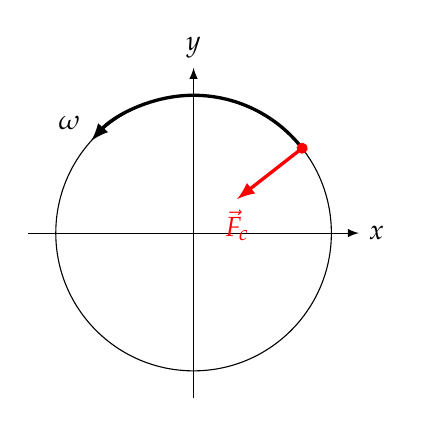
\begin{tikzpicture}[scale=.7]
      \draw[->](-3,0)--(3,0) node[right]{$x$};
      \draw[->](0,-3)--(0,3) node[above]{$y$};
      \draw circle(2.5);
      \begin{scope}[rotate=38]
        \begin{scope}[very thick,->]
          \draw[red] (2.45,0)--(1,0) node[below]{$\vec F_c$};
          \draw(2.5,0) arc(0:100:2.5) node[above left]{$\omega$};
        \end{scope}
        \fill[red] (2.5,0) circle(.1);
      \end{scope}
    \end{tikzpicture}

    \column{.7\textwidth}
    \begin{itemize}
    \item Centripetal force $\vec F_c$ is always perpendicular to the
      motion of the object
    \item $\vec F_c$ does not do any mechanical work
    \item Therefore, angular velocity $\vec\omega$ remains constant
    \item\textbf{The ``rotational state'' of the object does not change}
    \item Rotation of an object is not determined by merely what forces are
      acting it
    \end{itemize}
  \end{columns}
\end{frame}



\begin{frame}{Turning A Wrench}
  \begin{columns}
    \column{.3\textwidth}
    \pic{1.1}{wrench}
    
    \column{.7\textwidth}
    Similarly, when tightening/loosening a bolt by turning a wrench,
    \begin{itemize}
    \item When the nut turns, its ``rotational state'' changes
    \item The applied force has to be directed at a distance away from the
      bolt
    \item How easy to turn the nut depends on \emph{both} the distance and the
      force
    \end{itemize}
  \end{columns}
\end{frame}



\begin{frame}{Torque}
  Recall the second law of motion for objects with constant mass:
    
  \eq{-.1in}{
    \vec F_\text{net}=m\vec a
  }

  \vspace{-.1in}Is it also true for \emph{rotational} motion? If a net force
  $\vec F_\text{net}$ causes the center of mass of an object to begin to
  accelerate, what causes a mass to rotate?
\end{frame}



\begin{frame}{What is Torque?}
  \textbf{Torque} (or \textbf{moment}) is the tendency for a force to change
  the rotational motion of a body.
  \begin{itemize}
  \item A force $\vec F$ acting at a point some distance $\vec r$ (called the
    \textbf{moment arm}) from a \textbf{fulcrum} (or \textbf{pivot}) at an angle
    $\phi$ between $\vec F$ and $\vec r$
  \item e.g.\ the force to twist a screw
  \end{itemize}
  In the example below, a force $\vec F$ is applied $\vec r$ away from the pivot
  at an angle $\phi$. This generates a torque around the pivot.
  \begin{center}
    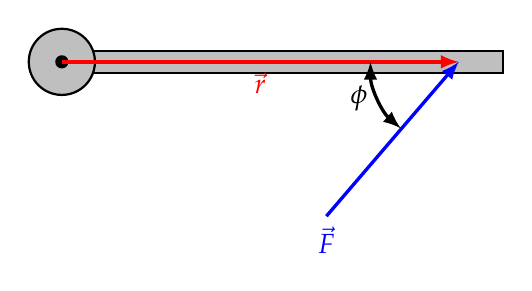
\begin{tikzpicture}[scale=2.8]
      \begin{scope}[thick]
        \draw[fill=lightgray](0,-.05) rectangle (2,.05);
        \draw[fill=lightgray] circle (.15);
      \end{scope}
      \fill circle (.03);
      \begin{scope}[very thick]
        \draw[red,->](0,0)--(1.8,0) node[midway,below]{$\vec r$};
        \draw[blue,->](1.2,-.7)--(1.8,0) node[pos=0,below]{$\vec F$};
        \draw[<->] (1.4,0) arc(180:229:.4)node[midway,left]{$\phi$};
      \end{scope}
    \end{tikzpicture}
  \end{center}
\end{frame}



\begin{frame}{Torque}
  Torque $\vec\tau$ is defined as the cross product of the force $\vec F$ and
  the \textbf{moment arm} $\vec r$. The unit for torque is a \textbf{newton
    meter} (\si{\newton\metre}).

  \eq{-.1in}{
    \boxed{\vec\tau=\vec r\times\vec F}
  }

  \vspace{-.1in}Its magnitude can be calculated in scalar form
  using the angle $\phi$ between $\vec F$ and $\vec r$:

  \eq{-.1in}{
    \boxed{\tau=Fr\sin\phi}
  }
  \begin{center}
    \begin{tabular}{l|c|c}
      \rowcolor{pink}
      \textbf{Quantity} & \textbf{Symbol} & \textbf{SI Unit} \\ \hline
      Torque        & $\vec\tau$ & \si{\newton\metre} \\
      Applied force & $\vec F$   & \si\newton \\
      Moment arm (from fulcrum to force) & $\vec r$ & \si\metre \\
      Angle between force and moment arm & $\phi$ & (no units)
    \end{tabular}
  \end{center}
\end{frame}



\begin{frame}{Example Problem}
  \textbf{Example:} Find the net torque on point C.
  \begin{center}
    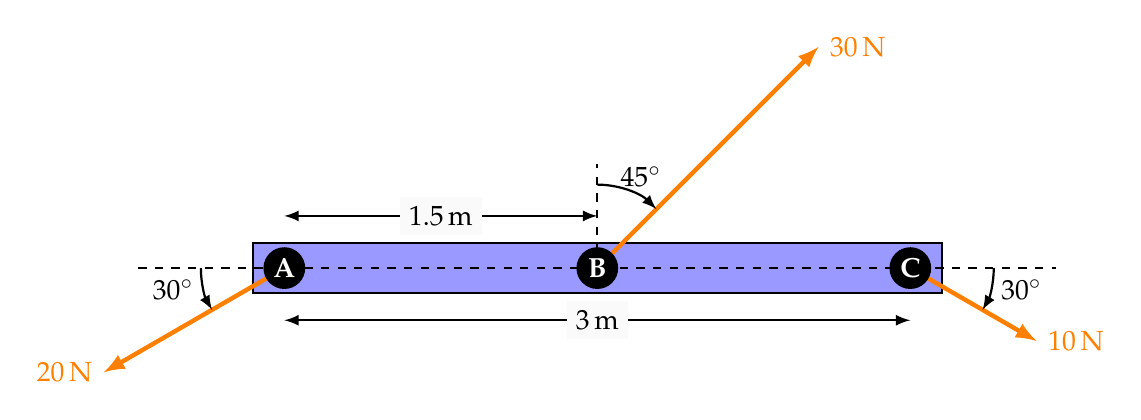
\begin{tikzpicture}[scale=2.65]
      \fill[blue!40,draw=black,thick] (-1.65,-.12) rectangle (1.65,.12);
      \draw[thick,<->](-1.5,-.25)--(1.5,-.25)
      node[midway,fill=black!2]{\SI{3.}\metre};
      \draw[thick,<->](-1.5,.25)--(0,.25)
      node[midway,fill=black!2]{\SI{1.5}\metre};
      \draw[dashed,thick](-2.2,0)--(2.2,0);
      \draw[dashed,thick](0,0)--(0,.5);
      \begin{scope}[orange,ultra thick,->]
        \draw[rotate=-45](0,0)--(0,1.5)node[right]{\SI{30}\newton};
        \draw[rotate around={30:(-1.5,0)}](-1.5,0)--(-2.5,0)
        node[left]{\SI{20}\newton};
        \draw[rotate around={-30:(1.5,0)}](1.5,0)--(2.2,0)
        node[right]{\SI{10}\newton};
      \end{scope}
      \begin{scope}[thick,->]
        \draw(0,.4)   arc(90:45:.4)  node[pos=.7,above]{\ang{45}};
        \draw(-1.9,0) arc(180:210:.4)node[midway,left] {\ang{30}};
        \draw(1.9,0)  arc(0:-30:.4)  node[midway,right]{\ang{30}};
      \end{scope}
      \fill (-1.5,0) circle(.1) node[white]{\textbf{A}};
      \fill (   0,0) circle(.1) node[white]{\textbf{B}};
      \fill ( 1.5,0) circle(.1) node[white]{\textbf{C}};
    \end{tikzpicture}
  \end{center}
\end{frame}





%%\begin{frame}{Torque}
%%  Going back to the example question:
%%  \begin{center}
%%    \begin{tikzpicture}
%%      \fill[black!75,draw=black!75] (-5,-.05) rectangle (5,.05);
%%      \fill (0,0) circle (.1);
%%      \draw[ultra thick](0,0)--(.5,-1.5)--(-.5,-1.5)--(0,0);
%%      \uncover<2->{
%%        \draw[ultra thick,red!75,->](0,0)--(-4.8,0) node[pos=.5,below]{$d_1$};
%%        \draw[ultra thick,red!75,->](-4.8,0)--(-4.8,-1)node[below]{$F_1$};
%%      }
%%      \uncover<3->{
%%        \draw[ultra thick,blue!60,->](0,0)--(4,0) node[pos=.5,below]{$d_2$};
%%        \draw[ultra thick,blue!60,->](4,0)--(4,-1.2) node[below]{$F_2$};
%%      }
%%    \end{tikzpicture}
%%  \end{center}
%%  \begin{itemize}
%%  \item<2->$F_1$ will rotate the board counter clockwise
%%  \item<3->$F_2$ will rotate the board clockwise
%%  \item<4->The beam will remain static (in equilibrium) if
%%
%%    \eq{-.2in}{ F_1d_1=F_2d_2 }
%%  \end{itemize}
%%\end{frame}



\section{Angular Momentum}

\begin{frame}{Angular Momentum}
  Consider a mass $m$ connected to a massless beam rotates with velocity
  $\vec v$ at a position $\vec r$ from the center (shown on the right). It has
  an \textbf{angular momentum} ($\vec L$), defined as:
  \begin{columns}
    \column{.77\textwidth}
    
    \eq{-.1in}{
      \boxed{\vec L=\vec r\times\vec p=m(\vec r\times\vec v)}
    }

    \vspace{-.1in}Expanding the term with $\vec v=\vec\omega\times\vec r$, the
    expression for angular momentum can now be expressed in quantities related
    to rotations:

    \eq{-.1in}{
      \boxed{\vec L=m(\vec r\times\vec v)
        =m(\vec r\times(\vec\omega\times\vec r))
        =mr^2\vec\omega}
    }
    
    \vspace{-.2in}Or in scalar form:
    
    \eq{-.1in}{
      \boxed{L=rmv=mr^2\omega}
    }

    \vspace{-.2in}The unit for angular momentum is a
    \textbf{kilogram meter squared per second}
    (\si{\newton\metre\squared\per\second}).
    
    \column{.23\textwidth}
    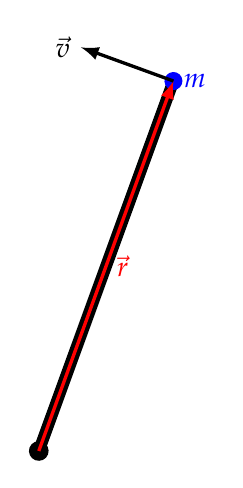
\begin{tikzpicture}[scale=2.5]
      \begin{scope}[rotate=70]
        \fill (0,-.03) rectangle (2,.03);
        \fill[blue,draw=blue,thick] (2,0) circle(.04) node[right]{$m$};
        \fill circle (.05);
        \begin{scope}[very thick,->]
          \draw[red](0,0)--(2,0)node[midway,right]{$\vec r$};
          \draw (2,0)--(2,.5)node[left]{$\vec v$};
        \end{scope}
      \end{scope}
    \end{tikzpicture}
  \end{columns}
\end{frame}



\begin{frame}{Moment of Inertia}
  Look again at the definition of angular momentum:
    
  \eq{-.1in}{
    \vec L=\underbrace{mr^2}_I\vec\omega
  }
    
  The quantity $I=mr^2$ is called the \textbf{moment of inertia} with a unit of
  \textbf{kilogram meter squared} (\si{\kilo\gram\metre\squared}), and 

  \eq{-.1in}{
    \boxed{\vec L=I\vec\omega}
  }

  Momentum of inertia can be considered to be an object's ``rotational mass''
\end{frame}



\begin{frame}{Moment of Inertia}
  For a \emph{single particle} of $m$ rotating at a distance $r$ from the pivot:
  
  \eq{-.1in}{
    \boxed{I=mr^2}
  }

  For a \emph{collection of particles} rotating at $\omega$, each of mass
  $m_i$ at distance $r_i$ from the pivot:

  \eq{-.1in}{
    \boxed{I=\sum m_ir_i^2}
  }

  For a \emph{continuous distribution of mass} rotating about a pivot, integral
  calculus is need to calculate the momentum of inertia:

  \eq{-.1in}{
    \boxed{I=\int r^2\dl m}
  }
\end{frame}



\begin{frame}{Moment of Inertia}
  \centering
  \pic{.7}{mic}
\end{frame}



\begin{frame}{Angular Momentum and Moment of Inertia}
  Linear and angular momentum have very similar expressions
    
  \vspace{-.3in}{\large
    \begin{align*}
      \vec p&=m\vec v\\
      \vec L&=I\vec\omega
    \end{align*}
  }
  
  Just as $\vec p$ describes the overall \emph{translational} state of motion
  of a physical system, $\vec L$ describes its overall \emph{rotational} state
\end{frame}



\section{Laws of Motion}

\begin{frame}{Equilibrium: First Law of Motion}
  An object is in \textbf{translational equilibrium} is when the net force
  acting on it is zero:
  
  \eq{-.1in}{
    \vec F_\text{net}=\vec 0
  }

  This does \emph{not} mean that the object has no translational motion; it
  just means that the object's overall \emph{transtational state} is not
  changing, i.e.\ momentum $\vec p$ is constant. For constant mass $m$,
  this means that $\vec a=\vec 0$.
\end{frame}




\begin{frame}{Equilibrium: First Law of Motion}
  Likewise, an object is in \textbf{rotational equilibrium} when the net torque
  acting on it is zero:

  \eq{-.1in}{
    \vec\tau_\text{net}=\vec 0
  }
  
  This does \emph{not} mean that the object has no rotational motion; it just
  means that the object's overall \emph{rotational state} is not changing,
  i.e.\  angular momentum $\vec L$ is constant. For constant moment of inertia
  $I$, this means that $\vec\alpha=\vec 0$.
\end{frame}



\begin{frame}{Second Law of Motion for Rotational Motion}
  The net torque is the time rate of change of angular momentum:

  \eq{-.1in}{
    \vec\tau_\text{net}=\vec r\times\vec F_\text{net}
    =\vec r\times\diff{\vec p}t
    =\diff{(\vec r\times\vec p)}t\;\;\longrightarrow\;\;
    \boxed{\vec\tau_\text{net}=\diff{\vec L}t}
  }
  \begin{itemize}
  \item If the net torque on a system is zero, then the rate of change
    of angular momentum is zero, and we say that the angular momentum is
    conserved. 
  \item e.g.\ When an ice skater starts to spin and draws his arms inward.
    Since angular momentum is conserved, a decrease in $r$ means an
    increase in $\omega$.
  \end{itemize}
\end{frame}



\begin{frame}{Second Law of Motion for Translational Motion}
  For translational motion, the general form of the first and second laws of
  motion states that the net force is rate of change of the object's momentum:

  \eq{-.1in}{
    \vec F_\text{net}=\diff{\vec p}t
  }

  For objects with constant mass, this reduces to the more familiar form:

  \eq{-.1in}{
    \vec F=m\vec a
  }
\end{frame}



\begin{frame}{Second Law of Motion for Rotational Motion}
  Likewise, the second law of motion for rotational motion has a similar form,
  but with torque $\vec\tau$ replacing force $\vec F$, and angular momentum
  $\vec L$ replacing linear momentum $\vec p$:

  \eq{-.1in}{
    \boxed{
      \vec\tau_\text{net}=\diff{\vec L}t
    }
  }

  For objects with constant momentum of inertia $I$, this reduces to:

  \eq{-.1in}{
    \boxed{
      \vec\tau_\text{net}=I\vec\alpha
    }
  }
\end{frame}



\begin{frame}{But there is no rotational motion, is there?}
  Even when there is no apparent rotational motion, it does not necessarily
  mean that angular momentum is zero! In this case, mass $m$ travels along a
  straight path at constant velocity (uniform motion), but the angular momentum
  around point $P$ is not zero:
  \begin{center}
    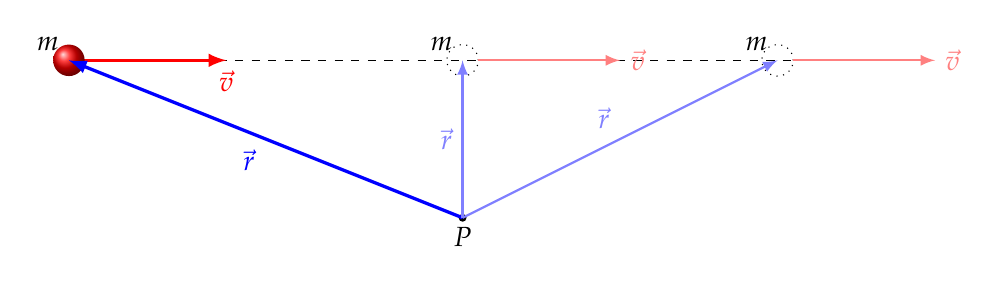
\begin{tikzpicture}
      \draw[dashed](-5,0)--(5,0);
      \draw[very thick,red,->](-5,0)--(-3,0) node[below]{$\vec v$};
      \shade[ball color=red] (-5,0) circle(.2) node[above left]{$m$};
      \fill (0,-2) circle(.05) node[below]{$P$};
      \draw[very thick,blue,->](0,-2)--(-5,0)
      node[midway,below left]{$\vec r$};
      \uncover<2->{
        \draw[dotted](0,0) circle(.2) node[above left]{$m$};
        \draw[thick,red!50,->](.2,0)--(2,0)node[right]{$\vec v$};
        \draw[thick,blue!50,->](0,-2)--(0,0) node[midway,left]{$\vec r$};
      }
      \uncover<3->{
        \draw[dotted](4,0) circle(.2) node[above left]{$m$};
        \draw[thick,red!50,->](4.2,0)--(6,0)node[right]{$\vec v$};
        \draw[thick,blue!50,->](0,-2)--(4,0)node[midway,above left]{$\vec r$};
      }
    \end{tikzpicture}
  \end{center}
  \uncover<4>{
    Since there is no force and no torque acting on the object, both the linear
    momentum ($\vec p=m\vec v$) and angular momentum
    ($\vec L=\vec r\times\vec v$) are constant.
  }
\end{frame}



\begin{frame}{Example Problem}
  \textbf{Example:} A skater extends her arms (both arms!), holding a
  \SI{2.}{\kilo\gram} mass in each hand. She is rotating about a vertical axis
  at a given rate. She brings her arms inward toward her body in such a way that
  the distance of each mass from the axis changes from \SI{1.}\metre to
  \SI{.50}\metre. Her rate of rotation (neglecting her own mass) will?
\end{frame}




\begin{frame}{Example Problem}
  \textbf{Example:} A \SI{1.}{\kilo\gram} mass swings in a vertical circle
  after having been released from a horizontal position with zero initial
  velocity. The mass is attached to a massless rigid rod of length
  \SI{1.5}\metre. What is the angular momentum of the mass, when it is in its
  lowest position?
\end{frame}
\end{document}
